% Usage: knitr slide


\chapter{Descriptive Statistics, Distributions, and Graphics}   \ros{2,5}\ems{3}
\section{Distributions} \ros{5.1-5.5}\katz{4}\abd{1.4}
The \emph{distribution} of a random variable $X$ is a profile of its
variability and other tendencies.
Depending on the type of $X$, a distribution is
characterized by the following.
\bi
\item Binary variable: the probability of ``yes'' or ``present'' (for
  a population) or the proportion of same (for a sample). \\
\item $k$-Category categorical (polytomous, multinomial) variable: the probability that a randomly chosen
  person in the population will be from category $i, i=1,\ldots,k$.
  For a sample, use $k$ proportions or percents.
\item Continuous variable: any of the following 4 sets of statistics
 \bi
 \item probability density: value of $x$ is on the $x$-axis, and the
   relative likelihood of observing a value ``close'' to $x$ is on the
   $y$-axis.  For a sample this yields a histogram.
 \item cumulative probability distribution: the $y$-axis contains the
   probability of observing $X\leq x$.  This is a function that is
   always rising or staying flat, never decreasing.  For a sample it
   corresponds to a cumulative histogram\footnote{But this
     \emph{empirical cumulative distribution function} can be drawn
     with no grouping of the data, unlike an ordinary histogram.}
 \item all of the \emph{quantiles} or \emph{percentiles} of $X$
 \item all of the \emph{moments} of $X$ (mean, variance, skewness,
   kurtosis, \ldots)
 \item If the distribution is characterized by one of the above four
   sets of numbers, the other three sets can be derived from this set
\ei
\item Ordinal Random Variables
  \bi
  \item Because there many be heavy ties, quantiles may not be good
    summary statistics
  \item The mean may be useful if the spacings have reasonable
    quantitative meaning
  \item The mean is especially useful for summarizing ordinal
    variables that are counts
  \item When the number of categories is small, simple proportions may
    be helpful
  \item With a higher number of categories, exceedance probabilities
    or the empirical cumulative distribution function are very useful
  \ei
\item Knowing the distribution we can make intelligent guesses about
  future observations from the same series, although unless the
  distribution really 
  consists of a single point there is a lot of uncertainty in
  predicting an individual new patient's response.  It is less
  difficult to predict the average response of a group of patients
  once the distribution is known.  
\item At the least, a distribution tells
  you what proportion of patients you would expect to see whose
  measurement falls in a given interval.
\ei

\subsection{Continuous Distributions}
\begin{Schunk}
\begin{Sinput}
x <- seq(-3, 35, length=150)
par(mfrow=c(1,2)); xl <- expression(x)   # Fig. (*\ref{fig:descript-pdfcdf}*):
plot(x, dt(x, 4, 6), type='l', xlab=xl, ylab='Probability Density Function')
plot(x, pt(x, 4, 6), type='l', xlab=xl, ylab='Cumulative Distribution Function')
\end{Sinput}
\begin{figure}[htbp]

\centerline{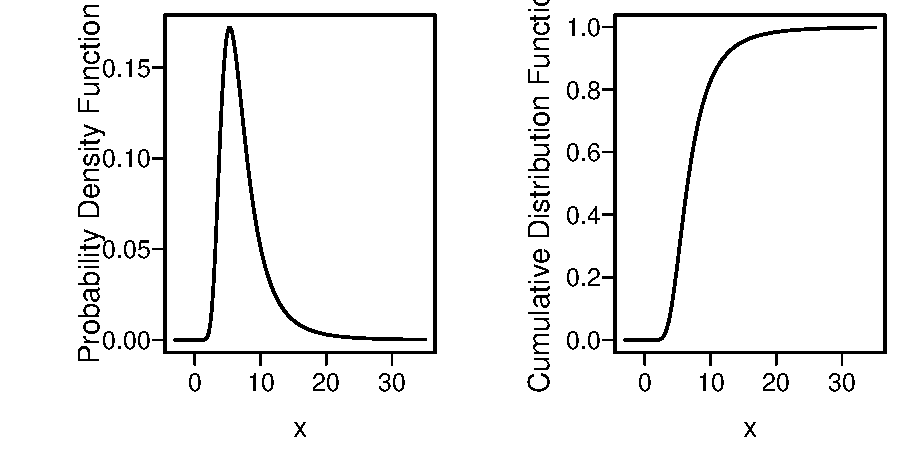
\includegraphics[width=\maxwidth]{descript-pdfcdf-1} }

\caption[Density and cumulative distribution functions]{Example probability density (a) and cumulative probability distribution (b) for a positively skewed random variable (skewed to the right)}\label{fig:descript-pdfcdf}
\end{figure}
\end{Schunk}

\begin{Schunk}
\begin{Sinput}
set.seed(1); x <- rnorm(1000)   # Fig. (*\ref{fig:descript-normalhist}*):
hist(x, nclass=40, prob=TRUE, col=gray(.9), xlab=xl, ylab='')
x <- seq(-4, 4, length=150)
lines(x, dnorm(x, 0, 1), col='blue', lwd=2)
\end{Sinput}
\begin{figure}[htbp]

\centerline{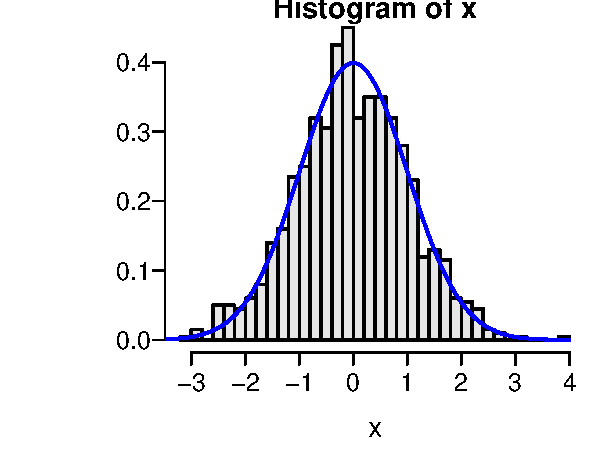
\includegraphics[width=\maxwidth]{descript-normalhist-1} }

\caption[Symmetric continuous distribution]{Example of a continuous distribution that is symmetric: the Gaussian (normal) distribution with mean 0 and variance 1, along with a histogram from a sample of size 1000 from this distribution}\label{fig:descript-normalhist}
\end{figure}
\end{Schunk}

\begin{Schunk}
\begin{Sinput}
set.seed(2)
x <- c(rnorm(500, mean=0, sd=1), rnorm(500, mean=6, sd=3))
hist(x, nclass=40, prob=TRUE, col=gray(.9), xlab=xl, ylab='')
lines(density(x), col='blue', lwd=2)
abline(v=c(0, 6), col='red')   # Fig. (*\ref{fig:descript-bimode}*)
\end{Sinput}
\begin{figure}[htbp]

\centerline{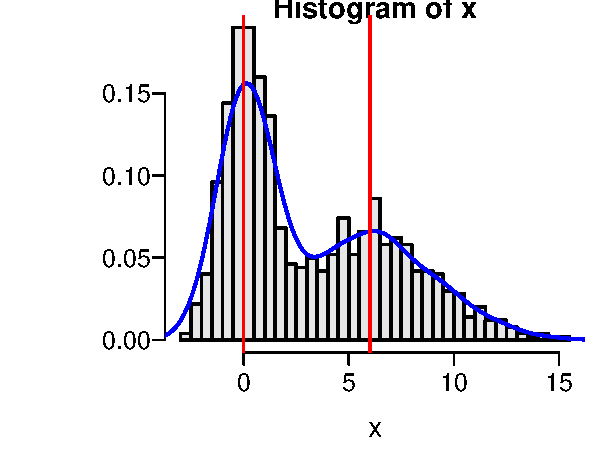
\includegraphics[width=\maxwidth]{descript-bimode-1} }

\caption[Bimodal distribution]{Example of a bimodal distribution from sampling from a mixture of normal distributions with different means and variances and estimating the underlying density function.  Vertical red lines indicate true population means of the two component populations.  Such a distribution can occur naturally or by failing to condition on a binary characteristic such as sex.}\label{fig:descript-bimode}
\end{figure}
\end{Schunk}

\subsection{Ordinal Variables}
\bi
\item Continuous ratio-scaled variables are ordinal
\item Not all ordinal variables are continuous or ratio-scaled
\item Best to analyze ordinal response variables using nonparametric tests or ordinal regression
\item Heavy ties may be present
\item Often better to treat count data as ordinal rather than to assume a distribution such as Poisson or negative binomial that is designed for counts
 \bi
 \item Poisson or negative binomial do not handle extreme clumping at zero
 \ei
\item Example ordinal variables are below
\ei

\begin{Schunk}
\begin{Sinput}
x <- 0:14
y <- c(.8, .04, .03, .02, rep(.01, 11))
plot(x, y, xlab=xl, ylab='', type='n')   # Fig. (*\ref{fig:descript-orda}*)
segments(x, 0, x, y)
\end{Sinput}
\begin{figure}[htbp]

\centerline{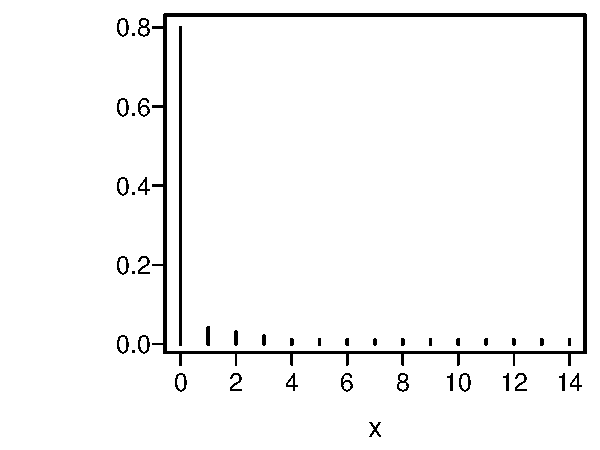
\includegraphics[width=\maxwidth]{descript-orda-1} }

\caption[Count variable with clumping at zero]{Distribution of number of days in the hospital in the year following diagnosis}\label{fig:descript-orda}
\end{figure}
\end{Schunk}
\begin{Schunk}
\begin{Sinput}
x <- 1:10
y <- c(.1, .13, .18, .19, 0, 0, .14, .12, .08, .06)
plot(x, y, xlab=xl, ylab='', type='n')   # Fig. (*\ref{fig:descript-ordb}*)
segments(x, 0, x, y)
\end{Sinput}
\begin{figure}[htbp]

\centerline{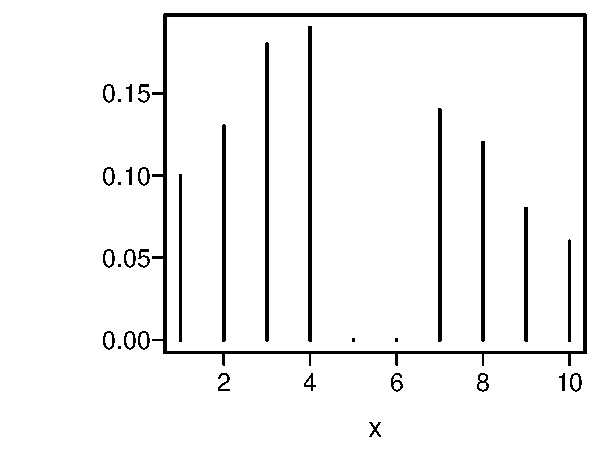
\includegraphics[width=\maxwidth]{descript-ordb-1} }

\caption[Ordinal variable with strange distribution]{Distribution of a functional status score that does not have points in the middle}\label{fig:descript-ordb}
\end{figure}
\end{Schunk}
The \co{getHdata} function in the \co{Hmisc} package~\cite{Hmisc}
finds, downloads, and \co{load()}s datasets from
\href{https://hbiostat.org/data}{hbiostat.org/data}.
\begin{Schunk}
\begin{Sinput}
require(Hmisc)
getHdata(nhgh)   # NHANES dataset    Fig. (*\ref{fig:descript-ordc}*):
scr <- pmin(nhgh$SCr, 5)   # truncate at 5 for illustration
scr[scr == 5 | runif(nrow(nhgh)) < .05] <- 5  # pretend 1/20 dialyzed
hist(scr, nclass=50, xlab='Serum Creatinine', ylab='Density', prob=TRUE)
\end{Sinput}
\begin{figure}[htbp]

\centerline{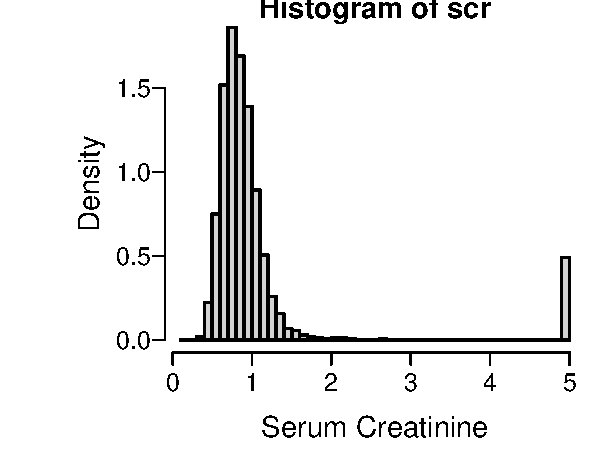
\includegraphics[width=\maxwidth]{descript-ordc-1} }

\caption[Continuous distribution with clumping at the end]{Distribution of serum creatinine where the patient requiring dialysis is taken to have the worst renal function.  The variable is mostly continuous but is best analyzed as ordinal so that no assumption is made about how to score dialysis except for being worse than all non-dialysis patients. Data taken from NHANES where no patients were actually dialyzed.}\label{fig:descript-ordc}
\end{figure}
\end{Schunk}
\clearpage
\section{Descriptive Statistics} \ros{2} \katz{4} \ems{3.2-3.3} \abd{3}
\subsection{Categorical Variables}
\bi
\item Proportions of observations in each category \\
  Note: The mean of a binary variable coded 1/0 is the proportion of
  ones.
\item For variables representing counts (e.g., number of
  comorbidities), the mean is a good summary measure (but not the median)
\item Modal (most frequent) category
\ei

\subsection{Continuous Variables} 
Denote the sample values as $x_{1}, x_{2}, \ldots, x_{n}$
\subsubsection{Measures of Location}
``Center'' of a sample
\bi
\item Mean: arithmetic average
\beq
\bar{x} = \frac{1}{n}\sum_{i=1}^{n}x_{i}
\eeq
Population mean $\mu$ is the long-run average (let $n \rightarrow
\infty$ in computing $\bar{x}$) \\
 \bi
 \item center of mass of the data (balancing point)
 \item highly influenced by extreme values even if they are highly
   atypical
 \ei
\item Median: middle sorted value, i.e., value such that $\frac{1}{2}$
  of the values are below it and above it
 \bi
 \item always descriptive
 \item unaffected by extreme values
 \item not a good measure of central tendency when there are heavy
   ties in the data
 \item if there are heavy ties and the distribution is limited or
   well-behaved, the mean often performs better than the median (e.g.,
   mean number of diseased fingers)
 \ei
\item Geometric mean: hard to interpret and affected by low outliers;
  better to use median
\ei

\subsubsection{Quantiles}
Quantiles are general statistics that can be used to describe central
tendency, spread, symmetry, heavy tailedness, and other quantities.
\bi
\item Sample median: the 0.5 quantile or $50^{th}$ percentile
\item Quartiles $Q_{1}, Q_{2}, Q_{3}$: 0.25 0.5 0.75 quantiles or
  $25^{th}, 50^{th}, 75^{th}$ percentiles
\item Quintiles: by 0.2
\item In general the $p$th sample quantile $x_{p}$ is the value such that a
  fraction $p$ of the observations fall below that value \\
\item $p^{th}$ population quantile: value $x$ such that the
  probability that $X \leq x$ is $p$
\ei

\subsubsection{Spread or Variability}
\bi
\item Interquartile range: $Q_{1}$ to $Q_{3}$ \\
Interval containing $\frac{1}{2}$ of the subjects \\
Meaningful for any continuous distribution
\item Other quantile intervals
\item Variance (for symmetric distributions): averaged squared
  difference between a randomly chosen observation and the mean of all
  observations
\beq
s^{2} = \frac{1}{n-1} \sum_{i=1}^{n} (x_{i} - \bar{x})^2
\eeq
The $-1$ is there to increase our estimate to compensate for our
estimating the center of mass from the data instead of knowing the
population mean.\footnote{$\bar{x}$ is the value of $\mu$ such that
  the sum of squared values about $\mu$ is a minimum.}
\item Standard deviation: $s$ --- $\sqrt{}$ of variance
 \bi 
 \item $\sqrt{}$ of average squared difference of an observation from
   the mean
 \item can be defined in terms of proportion of sample population within
   $\pm$ 1 SD of the mean \textbf{if the population is normal}
 \ei
\item SD and variance are not useful for very asymmetric data,
  e.g. ``the mean hospital cost was \$10000 $\pm$ \$15000''
\item Gini's mean difference: mean absolute difference over all
  possible pairs of observations.  This is highly interpretable. robust, and
  useful for all interval-scaled data, and is even highly precise if
  the data are normal\footnote{Gini's mean difference is labeled
    \co{Gmd} in the output of the \R\ \Co{Hmisc} \co{describe} function,
    and may be computed separately using the \Co{Hmisc} \co{GiniMd} function}.
\item range: not recommended because range $\uparrow$ as $n\uparrow$
  and is dominated by a single outlier
\item coefficient of variation: not recommended (depends too much on
  how close the mean is to zero)
\ei
Example of Gini's mean difference for describing patient-to-patient
variability of systolic blood pressure: If Gini's mean difference is
7mmHg, this means that the average disagreement (absolute difference)
between any two patients is 7mmHg.
\clearpage
\section{Graphics} \label{sec:graphics}\ros{2.8}\katz{4.2-4.6}\altman{17-20}\abd{2,3.4}\bmovie{3}\ddisc{3}
\movie{https://youtu.be/fSgEeI2Xpdc}
Cleveland~\cite{cle94ele,cle84sci} is the best source of how-to
information on making scientific graphs.  Much information may be
found at \url{https://biostat.app.vumc.org/StatGraphCourse},
especially these notes: \url{https://hbiostat.org/doc/graphscourse.pdf}.  Information about
graphics for reporting clinical trials may be found at
\href{http://biostat.app.vumc.org/RCTGraphics}{biostat.app.vumc.org/RCTGraphics}
and \href{https://hbiostat.org/R/hreport}{hbiostat.org/R/hreport}.  
A link to John Rauser's exceptional video about principles of good graphics
is found on that page as well as in the movie icon in the right margin.
See \href{https://discourse.datamethods.org/t/journal-graphics}{datamethods.org/t/journal-graphics} for graphical methods for journal articles.


Murrell~\cite{mur13inf} has an excellent summary of recommendations:
\begin{quote}
\bi
\item Display data values using position or length.
\item Use horizontal lengths in preference to vertical lengths.
\item Watch your data--ink ratio.
\item Think very carefully before using color to represent data
  values.
\item Do not use areas to represent data values.
\item \emph{Please} do not use angles or slopes to represent data
  values.
\item \emph{Please, please} do not use volumes to represent data
  values.
\ei
\end{quote}

On the fifth point above, avoid the use of \emph{bars} when
representing a single number.  Bar widths contain no information and
get in the way of important information.  This is addressed below.

\R\ has superior graphics implemented in multiple models, including
\bi
\item Base graphics such as \Co{plot(), hist(), lines(), points()}
  which give the user maximum control and are best used when not
  stratifying by additional variables other than the ones being summarized
\item The \Co{lattice} package which is fast but not quite as good as
  \Co{ggplot2} when one needs to vary more than one of color, symbol,
  size, or line type due to having more than one categorizing variable
\item The \Co{ggplot2} package which is very flexible and has the
  nicest defaults especially for constructing keys (legends/guides)
\item For semi-interactive graphics inserted into html reports, the
  \R\ \Co{plotly} package, which uses the \Co{plotly} system
  (which uses the Javascript \Co{D3} library) is extremely powerful.
  See \url{https://plot.ly/r/getting-started}. 
\item Fully interactive graphics can be built using \Co{RShiny} but
  this requires a server to be running while the graph is viewed.
\ei

For \Co{ggplot2}, \url{http://www.cookbook-r.com/Graphs} contains a
nice cookbook.  See also \url{http://learnr.wordpress.com}.  To get
excellent documentation with examples for any 
\Co{ggplot2} function, google \Co{ggplot2 \emph{functionname}}.
\Co{ggplot2} graphs can be converted into \Co{plotly} graphics using
the \Co{ggplotly} function.  But you will have more control using
\R\ \Co{plotly} directly.

The older non-interactive graphics models which are useful for
producing printed and \Co{pdf} output are starting to be superceded
with interactive graphics.  One of the biggest advantages of the
latter is the ability to present the most important graphic
information front-and-center but to allow the user to easily hover the
mouse over areas in the graphic to see tabular details.


\subsection{Graphing Change vs.\ Raw Data}\alabel{sec:descript-change}
A common mistake in scientific graphics is to cover up subject
variability by normalizing repeated measures for baseline (see
Section~\ref{sec:overview-preprocessing}).  Among other problems, this
prevents the reader from seeing regression to the mean for subjects
starting out at very low or very high values, and from seeing
variation in intervention effect as a function of baseline values.  It
is highly recommended that all the raw data be shown, including those
from time zero.  When the sample size is not huge, spaghetti plots are
most effective for graphing longitudinal data because all points from
the same subject over time are connected.  An
example~\citep{davis-repmeas}{pp.\ 161-163} is below. 
\begin{Schunk}
\begin{Sinput}
require(Hmisc)   # also loads ggplot2
getHdata(cdystonia)
ggplot(cdystonia, aes(x=week, y=twstrs, color=factor(id))) +
       geom_line() + xlab('Week') + ylab('TWSTRS-total score') +
       facet_grid(treat ~ site) +
       guides(color=FALSE) # Fig. (*\ref{fig:descript-spaghetti}*)
\end{Sinput}
\begin{figure}[htbp]

\centerline{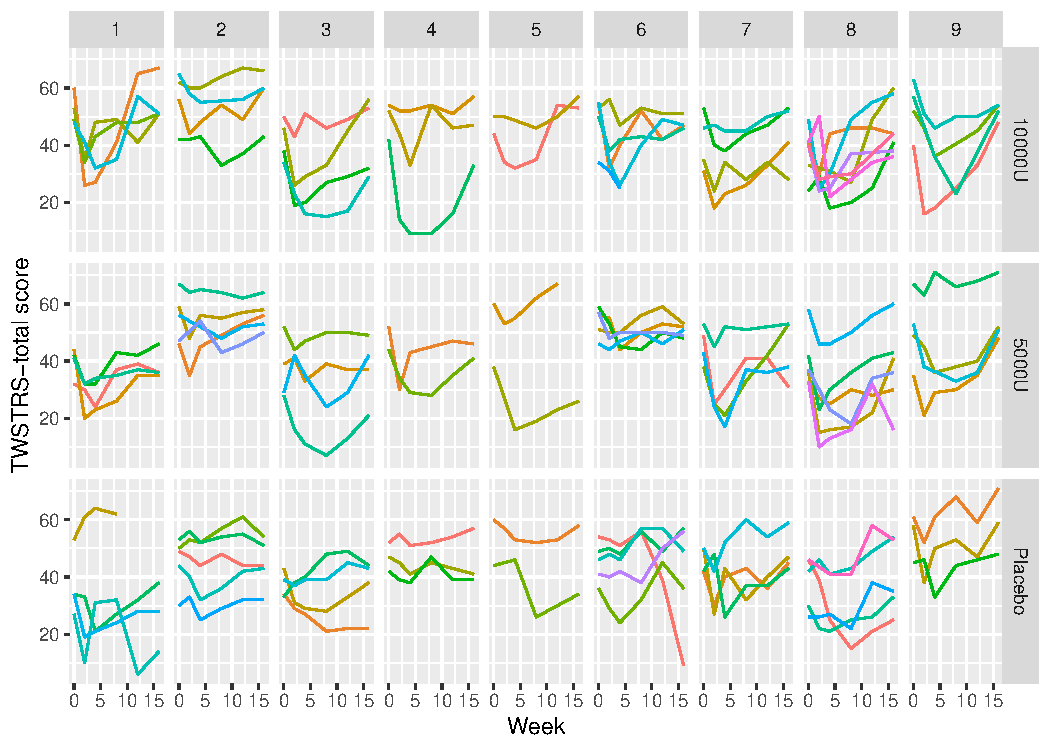
\includegraphics[width=\maxwidth]{descript-spaghetti-1} }

\caption[Spaghetti plot]{Spaghetti plot showing all the raw data on the response variable for each subject, stratified by dose and study site (1--9).  Importantly, week 0 (baseline) measurements are included.}\label{fig:descript-spaghetti}
\end{figure}
\end{Schunk}
Graphing the raw data is usually essential.

\subsection{Categorical Variables}
\bi
\item pie chart
 \bi
 \item high ink:information ratio
 \item optical illusions (perceived area or angle depends on
   orientation vs.\ horizon)
 \item hard to label categories when many in number
 \ei
\item bar chart
 \bi
 \item high ink:information ratio
 \item hard to depict confidence intervals (one sided error bars?)
 \item hard to interpret if use subcategories
 \item labels hard to read if bars are vertical
 \ei
\item dot chart
 \bi
 \item leads to accurate perception
 \item easy to show all labels; no caption needed
 \item allows for multiple levels of categorization (see Figures \ref{fig:descript-counts-dotchart} and \ref{desc-proportions-txreg})
 
\begin{Schunk}
\begin{Sinput}
getHdata(titanic3)
d <- upData(titanic3,
            agec     = cut2(age, c(10, 15, 20, 30)), print=FALSE)
d <- with(d, as.data.frame(table(sex, pclass, agec)))
d <- subset(d, Freq > 0)
ggplot(d, aes(x=Freq, y=agec)) + geom_point() +
  facet_grid(sex ~ pclass) +
  xlab('Frequency') + ylab('Age')
\end{Sinput}
\begin{figure}[htbp]

\centerline{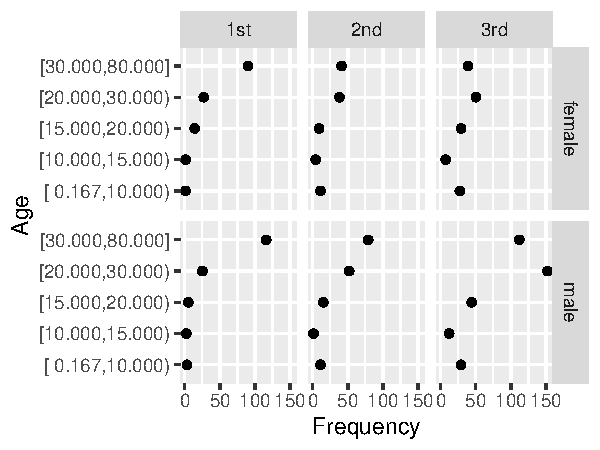
\includegraphics[width=\maxwidth]{descript-counts-dotchart-1} }

\caption[Frequency dot chart]{Dot chart showing frequencies from cross-classifications of discrete variables for Titanic passengers}\label{fig:descript-counts-dotchart}
\end{figure}
\end{Schunk}

\figs{desc-proportions-txreg}{Dot chart for categorical demographic
  variables, stratified by treatment and region}{1}

\figs{aevents}{Dot chart showing proportion of subjects having adverse
  events by treatment, sorted by risk difference, produced by the \R\
  \co{greport} package.  See \co{test.Rnw}
  at \protect\url{hbiostat.org/R/greport}}{1}

  \bi
  \item multi-panel display for multiple major categorizations
  \item lines of dots arranged vertically within panel
  \item categories within a single line of dots
  \ei
 \item easy to show 2-sided error bars
 \ei
\item Avoid chartjunk such as dummy dimensions in bar charts, rotated
  pie charts, use of solid areas when a line suffices
\ei

\subsection{Continuous Variables}
\subsubsection{Raw Data}
For graphing two continuous variable, scatterplots are often
essential.  The following example draws a scatterplot on a very large
number of observations in a measurement comparison study where the
goal is to measure esophageal pH longitudinally and across subjects.
\begin{Schunk}
\begin{Sinput}
getHdata(esopH)
contents(esopH)
\end{Sinput}
\begin{Soutput}

Data frame:esopH	136127 observations and 2 variables    Maximum # NAs:0


                                       Labels   Class Storage
orophar Esophageal pH by Oropharyngeal Device numeric  double
conv     Esophageal pH by Conventional Device numeric  double
\end{Soutput}
\begin{Sinput}
xl <- label(esopH$conv)
yl <- label(esopH$orophar)
ggplot(esopH, aes(x=conv, y=orophar)) + geom_point(pch='.') +
  xlab(xl) + ylab(yl) +   # Fig. (*\ref{fig:descript-pH}*)
  geom_abline(intercept = 0, slope = 1)
\end{Sinput}
\begin{figure}[htbp]

\centerline{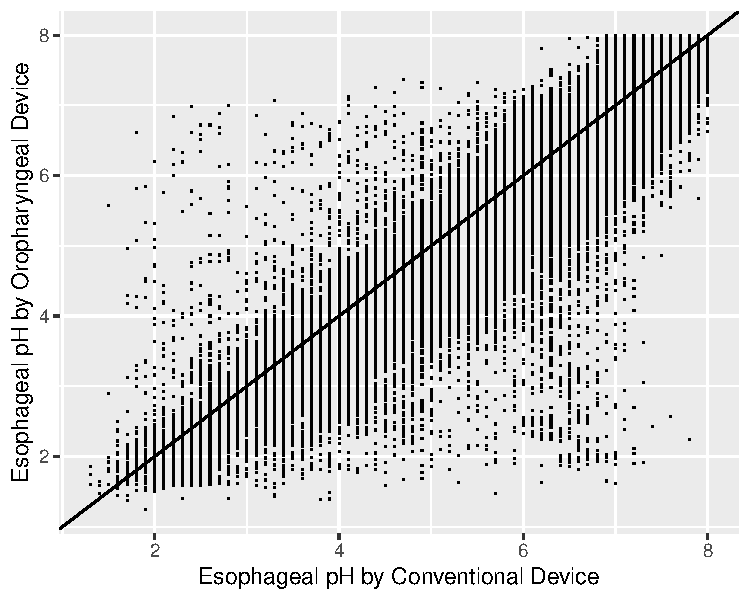
\includegraphics[width=\maxwidth]{descript-pH-1} }

\caption[Scatterplot of one measurement mode against another]{Scatterplot of one measurement mode against another}\label{fig:descript-pH}
\end{figure}
\end{Schunk}
With large sample sizes there are many collisions of data points and
hexagonal binning is an effective substitute for the raw
data scatterplot.  The number of points represented by one hexagonal
symbol is stratified into 20 groups of approximately equal numbers of
points.  The code below is not currently working for the \co{ggplot2}
package version 2.1.0. 
\begin{Schunk}
\begin{Sinput}
ggplot(esopH, aes(x=conv, y=orophar)) +
  stat_binhex(aes(alpha=..count.., color=Hmisc::cut2(..count.., g=20)),
              bins=80) +
  xlab(xl) + ylab(yl) +
  guides(alpha=FALSE, fill=FALSE, color=guide_legend(title='Frequency'))
\end{Sinput}
\end{Schunk}
Instead we use the \Co{Hmisc} \co{ggfreqScatter} function to bin the
points and represent frequencies of overlapping points with color and
transparency levels. 
\begin{Schunk}
\begin{Sinput}
with(esopH, ggfreqScatter(conv, orophar, bins=50, g=20) +
              geom_abline(intercept=0, slope=1))   # Fig. (*\ref{fig:descript-pHh2}*)
\end{Sinput}
\begin{figure}[htbp]

\centerline{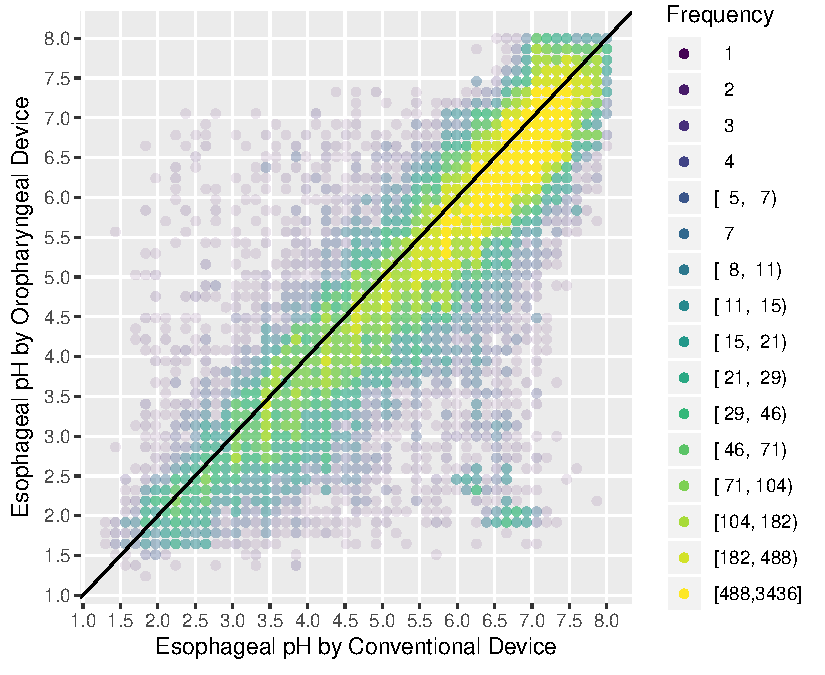
\includegraphics[width=\maxwidth]{descript-pHh2-1} }

\caption[Binned points (2500 total bins) with frequency counts shown as color and transparency level]{Binned points (2500 total bins) with frequency counts shown as color and transparency level}\label{fig:descript-pHh2}
\end{figure}
\end{Schunk}

\subsubsection{Distributions}\abd{1.4}\label{sec:desc-dist}
\bi
\item histogram showing relative frequencies
 \bi
 \item requires arbitrary binning of data
 \item not optimal for comparing multiple distributions
 \ei
\item cumulative distribution function: proportion of values $\leq x$
  vs.\ $x$ (Figure \ref{fig:descript-ecdf}) \\
 Can read all quantiles directly off graph.
\begin{Schunk}
\begin{Sinput}
getHdata(pbc)
pbcr <- subset(pbc, drug != 'not randomized')
Ecdf(pbcr[,c('bili','albumin','protime','sgot')],  # Fig. (*\ref{fig:descript-ecdf}*)
    group=pbcr$drug, col=1:2,
    label.curves=list(keys='lines'))
\end{Sinput}
\begin{figure}[htbp]

\centerline{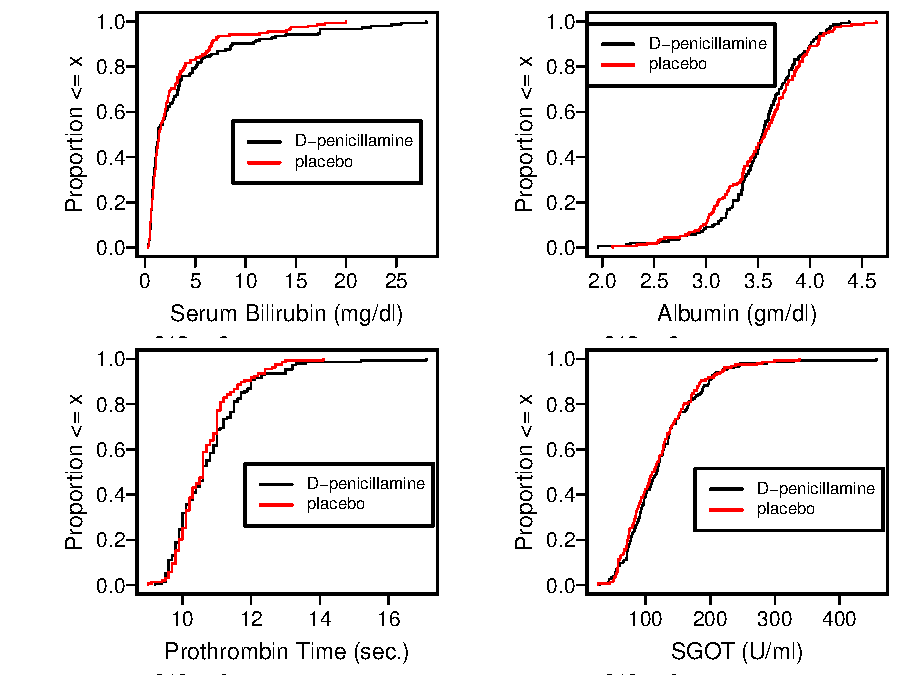
\includegraphics[width=\maxwidth]{descript-ecdf-1} }

\caption[Empirical cumulative distribution functions]{Empirical cumulative distributions of baseline variables  stratified by treatment in a randomized controlled trial. $m$ is the number of missing values.}\label{fig:descript-ecdf}
\end{figure}
\end{Schunk}

\item Box plots shows quartiles plus the mean.  They are a good way to
  compare many groups as seen in Figures~\ref{fig:descript-bwplot} and
  \ref{fig:descript-glybox}. 
\begin{Schunk}
\begin{Sinput}
getHdata(support)   # Fig. (*\ref{fig:descript-bwplot}*)
bwplot(dzgroup ~ crea, data=support, panel=panel.bpplot,
       probs=c(.05,.25), xlim=c(0,8), xlab='Serum Creatinine')
\end{Sinput}
\begin{figure}[htbp]

\centerline{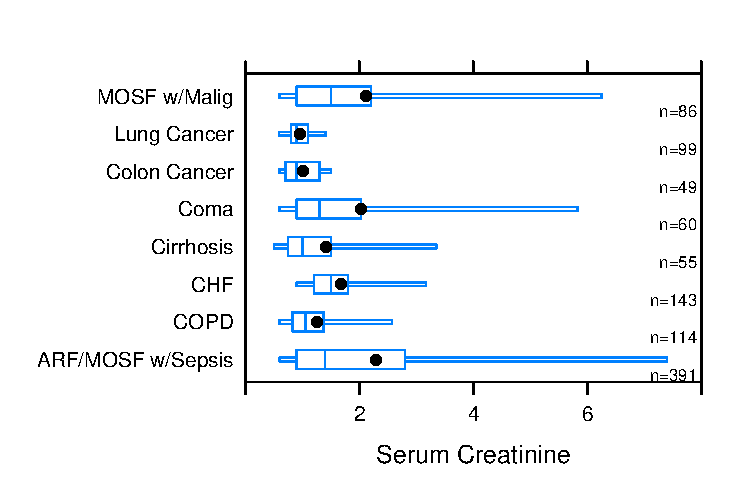
\includegraphics[width=\maxwidth]{descript-bwplot-1} }

\caption[Box plots with 0.05 and 0.95 quantiles]{Box plots showing the distribution of serum creatinine  stratified by major diagnosis.  Dot: mean; vertical line: median; large box:interquartile range.  The 0.05 and 0.95 quantiles are also shown, which is not the way typical box plots are drawn but is perhaps more useful.  Asymmetry of distributions can be seen by both disagreement between $Q_{3}-Q_{2}$ and $Q_{2}-Q_{1}$ and by disagreement between $Q_{2}$ and $\bar{x}$.}\label{fig:descript-bwplot}
\end{figure}
\end{Schunk}

Figure \ref{fig:descript-glybox} uses extended box plots.  The
following schematic shows how to interpret them.
\begin{Schunk}
\begin{Sinput}
bpplt()   # Fig. (*\ref{fig:descript-bpplt}*)
\end{Sinput}
\begin{figure}[htbp]

\centerline{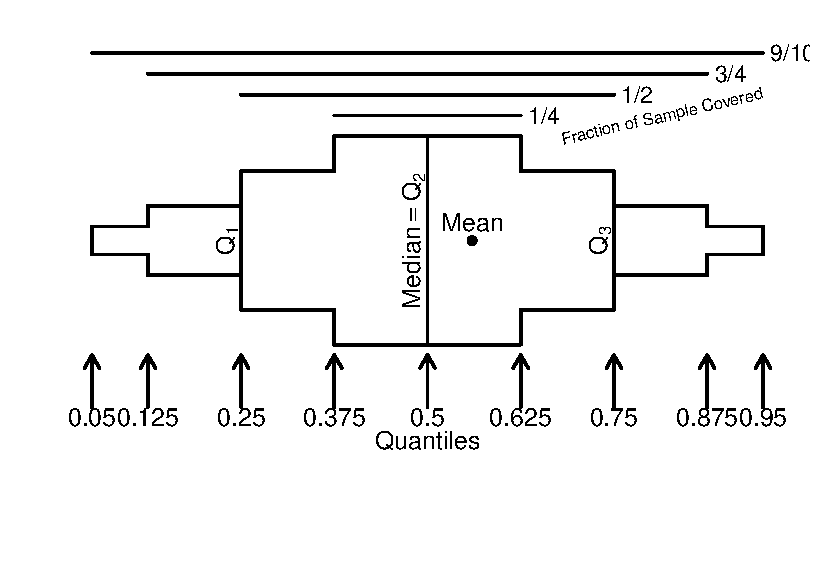
\includegraphics[width=\maxwidth]{descript-bpplt-1} }

\caption[Schematic for extended box plot]{Schematic for extended box plot}\label{fig:descript-bpplt}
\end{figure}
\end{Schunk}

\begin{Schunk}
\begin{Sinput}
require(lattice)   # Fig. (*\ref{fig:descript-glybox}*):
getHdata(diabetes)
wst <- cut2(diabetes$waist, g=2)
levels(wst) <- paste('Waist', levels(wst))
bwplot(cut2(age,g=4) ~ glyhb | wst*gender, data=diabetes,
       panel=panel.bpplot, xlab='Glycosylated Hemoglobin', ylab='Age Quartile')
\end{Sinput}
\begin{figure}[htbp]

\centerline{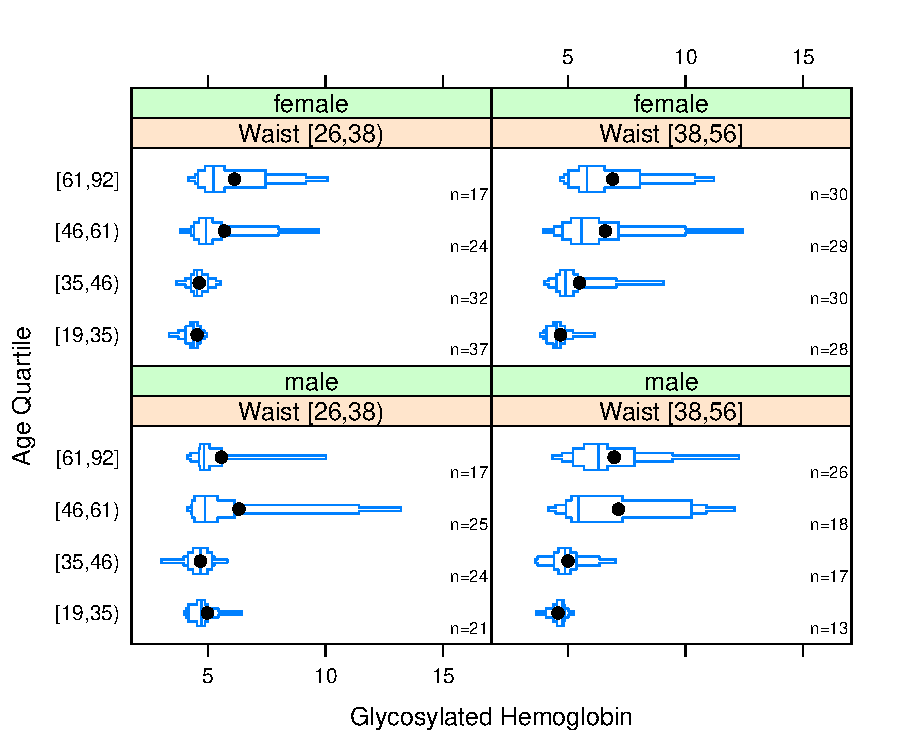
\includegraphics[width=\maxwidth]{descript-glybox-1} }

\caption[Extended box plots for glycohemoglobin]{Extended box plots for glycohemoglobin stratified by quartiles of age (vertical), two-tiles of waist circumference (horizontal), and sex (vertical)}\label{fig:descript-glybox}
\end{figure}
\end{Schunk}

Box plots are inadequate for displaying bimodality.  Violin plots show
the entire distribution well if the variable being summarized is
fairly continuous.

\figs{cchem-byx-cont-a}{One-half violin plots for longitudinal data, stratified
  by treatment.  Density estimates for groups with insufficient sample
  sizes are faded.  Density plots are back--to--back for treatment A
  and B.  Points are treatment medians.  When the black vertical line
  does not touch the two medians, the medians are significantly
  different at the $\alpha=0.05$ level.  Graphic was produced by the
  \R\ \Co{greport} package.}{1}
\ei


\subsubsection{Relationships}
\bi
\item When response variable is continuous and descriptor
  (stratification) variables are categorical, multi-panel dot charts,
  box plots, multiple cumulative distributions, etc., are useful.
\item Two continuous variables: scatterplot\ems{~Figure~3.9}
% also Rosner Figure 2.12
\ei


\subsection{Graphs for Summarizing Results of Studies}
\bi
\item Dot charts with optional error bars (for confidence limits) can
  display any summary statistic (proportion, mean, median, mean
  difference, etc.)
\item It is not well known that the confidence interval for a
  difference in two means cannot be derived from individual confidence
  limits.\footnote{In addition, it is not necessary for two confidence
    intervals to be separated for the difference in means to be
    significantly different from zero.} \\
  Show individual confidence limits as well as actual CLs for the
  difference.
\begin{Schunk}
\begin{Sinput}
attach(diabetes)
set.seed(1)
male   <- smean.cl.boot(glyhb[gender=='male'],   reps=TRUE)
female <- smean.cl.boot(glyhb[gender=='female'], reps=TRUE)
dif <- c(mean=male['Mean']-female['Mean'],
         quantile(attr(male, 'reps')-attr(female,'reps'), c(.025,.975)))
plot(0,0,xlab='Glycated Hemoglobin',ylab='',   # Fig. (*\ref{fig:descript-cldif}*)
     xlim=c(5,6.5),ylim=c(0,4), axes=F)
axis(1, at=seq(5, 6.5, by=0.25))
axis(2, at=c(1,2,3.5), labels=c('Female','Male','Difference'),
     las=1, adj=1, lwd=0)
points(c(male[1],female[1]), 2:1)
segments(female[2], 1, female[3], 1)
segments(male[2], 2,   male[3], 2)
offset <- mean(c(male[1],female[1])) - dif[1]
points(dif[1] + offset, 3.5)
segments(dif[2]+offset, 3.5, dif[3]+offset, 3.5)
at <- c(-.5,-.25,0,.25,.5,.75,1)
axis(3, at=at+offset, label=format(at))
segments(offset, 3, offset, 4.25, col=gray(.85))
abline(h=c(2 + 3.5)/2, col=gray(.85))
\end{Sinput}
\begin{figure}[htbp]

\centerline{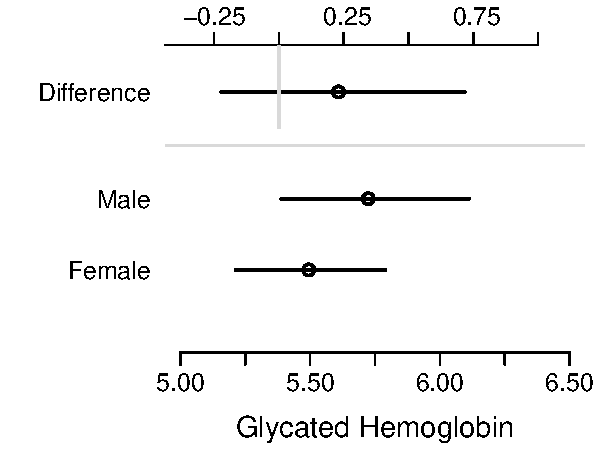
\includegraphics[width=\maxwidth]{descript-cldif-1} }

\caption[Showing group means and differences]{Means and nonparametric bootstrap 0.95 confidence limits for glycated hemoglobin for males and females, and confidence limits for males - females.  Lower and upper $x$-axis scales have same spacings but different centers.  Confidence intervals for differences are generally wider than those for the individual constituent variables.}\label{fig:descript-cldif}
\end{figure}
\end{Schunk}
  
\item For showing relationship between two continuous variables, a
  trend line or regression model fit, with confidence bands
\ei

\subsubsection{Bar Plots with Error Bars}

\bi
\item ``Dynamite'' Plots
\item Height of bar indicates mean, lines represent standard error
\item High ink:information ratio
\item Hide the raw data, assume symmetric confidence intervals
\item Replace with
  \bi
   \item Dot plot (smaller sample sizes)
   \item Box plot (larger sample size)
  \ei
\ei
\begin{Schunk}
\begin{Sinput}
getHdata(FEV); set.seed(13)   
FEV <- subset(FEV, runif(nrow(FEV)) < 1/8)   # 1/8 sample
require(ggplot2)
s <- with(FEV, summarize(fev, llist(sex, smoke), smean.cl.normal))
ggplot(s, aes(x=smoke, y=fev, fill=sex)) +    # Fig. (*\ref{fig:descript-dynamite}*)
    geom_bar(position=position_dodge(), stat="identity") +
    geom_errorbar(aes(ymin=Lower, ymax=Upper),
                  width=.1,
                  position=position_dodge(.9))
\end{Sinput}
\begin{figure}[htbp]

\centerline{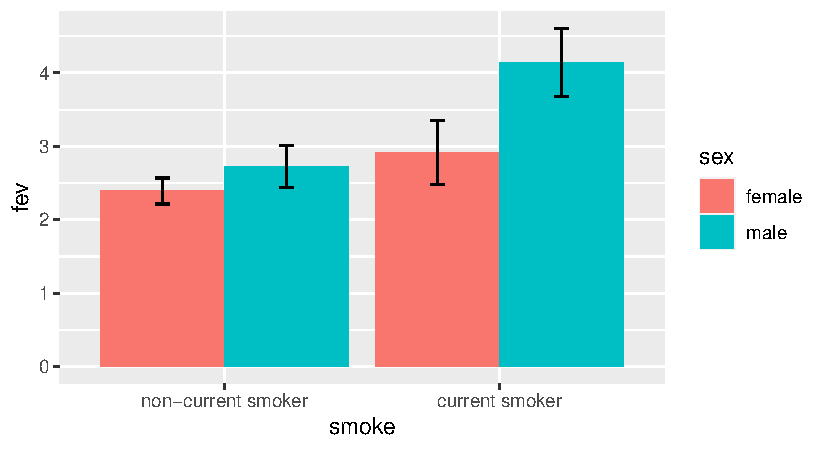
\includegraphics[width=\maxwidth]{descript-dynamite-1} }

\caption[Bar plot with error bars---``dynamite plot'']{Bar plot with error bars---``dynamite plot''}\label{fig:descript-dynamite}
\end{figure}
\end{Schunk}
See \url{http://biostat.app.vumc.org/DynamitePlots} for a list of
the many problems caused by dynamite plots, plus some solutions.

Instead of the limited information shown in the bar chart, show the
raw data along with box plots.  Modify default box plots to replace
whiskers with the interval between 0.1 and 0.9 quantiles.
\begin{Schunk}
\begin{Sinput}
require(ggplot2)   # Fig. (*\ref{fig:descript-tplot}*)
stats <- function(x) {
  z <- quantile(x, probs=c(.1, .25, .5, .75, .9))
  names(z) <- c('ymin', 'lower', 'middle', 'upper', 'ymax')
  if(length(x) < 10) z[c(1,5)] <- NA
  z
}
ggplot(FEV, aes(x=sex, y=fev)) +
  stat_summary(fun.data=stats, geom='boxplot', aes(width=.75), shape=5,
               position='dodge', col='lightblue') +
  geom_dotplot(binaxis='y', stackdir='center', position='dodge', alpha=.4) +
  stat_summary(fun.y=mean, geom='point', shape=5, size=4, color='blue') +
  facet_grid(~ smoke) +
  xlab('') + ylab(expression(FEV[1])) + coord_flip()
\end{Sinput}
\begin{figure}[htbp]

\centerline{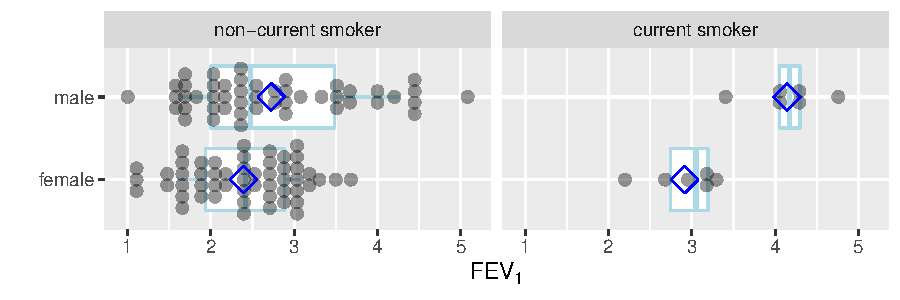
\includegraphics[width=\maxwidth]{descript-tplot-1} }

\caption[Dot plot with superimposed box plots]{Jittered raw data and box plots.  Middle vertical lines indicate medians and diamonds indicate means. Horizontal lines indicate 0.1 to 0.9 quantiles when $n\geq 10$.  The ink:information ratio for this plot is far better than a dynamite plot.}\label{fig:descript-tplot}
\end{figure}
\end{Schunk}
Use a violin plot to show the distribution density estimate (and its
mirror image) instead of a box plot.
\begin{Schunk}
\begin{Sinput}
ggplot(FEV, aes(x=sex, y=fev)) +
  geom_violin(width=.6, col='lightblue') +
  geom_dotplot(binaxis='y', stackdir='center', position='dodge', alpha=.4) +
  stat_summary(fun.y=median, geom='point', color='blue', shape='+', size=12) +
  facet_grid(~ smoke) +
  xlab('') + ylab(expression(FEV[1])) + coord_flip()
\end{Sinput}
\begin{figure}[htbp]

\centerline{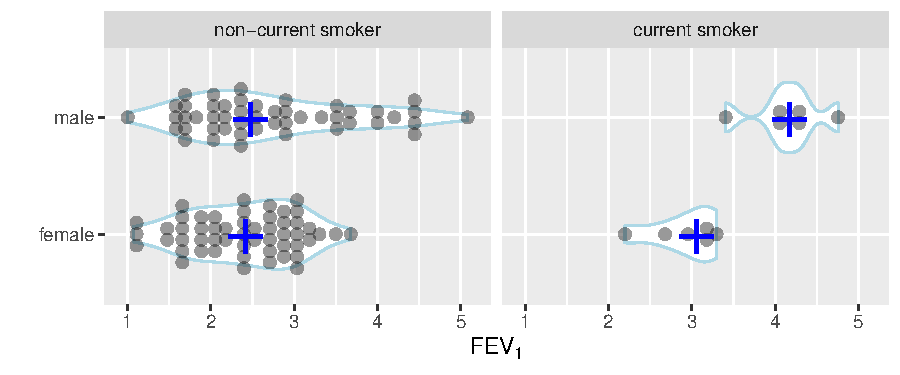
\includegraphics[width=\maxwidth]{descript-vplot-1} }

\caption[Jittered raw data and violin plots with median indicated by \textbf{\textcolor{blue}{+}}]{Jittered raw data and violin plots with median indicated by \textbf{\textcolor{blue}{+}}}\label{fig:descript-vplot}
\end{figure}
\end{Schunk}

% Was
% ggplot(FEV, aes(x=smoke, y=fev, color=sex)) +
%   geom_boxplot(alpha=.5, width=.2) + # remove width to overlay boxes on pts
%   stat_summary(fun.y=mean, geom="point", shape=5, size=2, 
%                position=position_dodge(width=.15)) +
%   geom_dotplot(binaxis='y', stackdir='center', position='dodge') +
%   xlab('') + ylab(expression(FEV[1])) + coord_flip() 
% ggplot(FEV, aes(x=smoke, y=fev, color=sex)) +
%   stat_summary(fun.data=stats, geom='boxplot', shape=5, position='dodge') +
%   geom_dotplot(binaxis='y', stackdir='center', position='dodge') +
%   stat_summary(fun.y=mean, geom="point", shape=5, size=2, 
%                position=position_dodge(width=.2)) +
%   xlab('') + ylab(expression(FEV[1])) + coord_flip()
  
%## Define Tatsuki Koyama's tplot function
%base <- 'http://biostat.mc.vanderbilt.edu/wiki/pub/Main'
%source(paste(base, 'TatsukiRcode/TatsukiRcodeTplot.R', sep='/'))
%par(mar=c(4,9,1,4))
%tplot(fev ~ smoke, data=FEV, show.n=TRUE, bty='L', type='db',
%      pch=20, las=1, mean.line=TRUE, horizontal=TRUE, ylab='FEV1',
%      col=c(female='darkred',male='darkblue')[as.character(FEV$sex)],
%      dist=.02, boxcol='lightyellow1', boxborder=gray(.8))  # Fig. (*\ref{fig:descript-tplot}*)

\subsubsection{Semi-Interactive Graphics Examples}

These examples are all found in \url{hbiostat.org/talks/rmedicine19.html}.

\bi
\item \href{https://hbiostat.org/talks/rmedicine19.html}{R for
  Clinical Trial Reporting}
\item \href{https://hbiostat.org/talks/rmedicine19.html#11}{Spike
  histograms with hovertext for overall statistical summary} (slide 11)
\item \href{https://hbiostat.org/talks/rmedicine19.html#12}{Dot plots}
  (slide 12)
\item \href{https://hbiostat.org/talks/rmedicine19.html#13}{Extended
  box plots} (slide 13)
\item \href{https://hbiostat.org/talks/rmedicine19.html#15}{Spike
  histograms with quantiles, mean, dispersion} (slide 15)
\item \href{https://hbiostat.org/talks/rmedicine19.html#16}{Survival
  plots with CI for difference, continuous number at risk} (slide 16)
\item \href{https://hbiostat.org/talks/rmedicine19.html#35}{Example
  clinical trial reports} (slide 35)
\ei

Other examples: descriptions of BBR course participants: \href{https://hbiostat.org/bbr/registrants.html}{hbiostat.org/bbr/registrants.html}.


\subsection{Graphs for Describing Statistical Model Fits}
Several types of graphics are useful.  These are all implemented in
the \R\ \Co{rms} package~\cite{rrms}.
\begin{description}
  \item[Partial effect plots]: Show the effect on $Y$ of varying one
    predictor at a time, holding the other predictors to medians or
    modes, and include confidence bands.  This is the best approach
    for showing shapes of effects of continuous predictors.
  \item[Effect charts]: Show the difference in means, odds ratio,
    hazard ratio, fold change, etc., varying each predictor and
    holding others to medians or modes\footnote{It does not matter
      what the other variables are set to if they do not interact with
      the variable being varied.}.  For continuous variables that do
    not operate linearly, this kind of display is not very
    satisfactory because of its strong dependence on the settings over
    which the predictor is set.  By default inter-quartile-range
    effects are used.
  \item[Nomograms]: Shows the entire model if the number of
    interactions is limited.  Nomograms show strengths and shapes of
    relationships, are very effective for continuous predictors, and
    allow computation of predicted values (although without confidence limits).
\end{description}
Here are examples using NHANES data to predict glycohemoglobin from
age, sex, race/ethnicity, and BMI.\\
\textbf{Note}: ordinary regression is not an adequate fit for glycohemoglobin;
an excellent fit comes from ordinal regression.  BMI is not an
adequate summary of body size.  The following
ordinary regression model in the $-1.75$ power of glycohemoglobin
resulted in approximately normal residuals and is used for
illustration.  The transformation is subtracted from a constant just
so that positive regression coefficients indicate that increasing a
predictor increases glycohemoglobin.  The inverse transformation
raises predicted values to 
the $-\frac{1}{1.75}$ power after accounting for the subtraction, and
is used to estimate the median glycohemoglobin on 
the original scale\footnote{If residuals have a normal distribution
  after transforming the dependent variable, the estimated mean and
  median transformed values are the same.  Inverse transforming the
  estimates provides an estimate of the median on the original scale
  (but not the mean).}.  Restricted cubic spline 
functions with 4 default 
knots are used to allow age and BMI to act smoothly but nonlinearly.
Partial effects plots are in Fig.~\ref{fig:descript-rmsa}.
\begin{Sinput}
require(rms)
getHdata(nhgh)   # NHANES data
dd <- datadist(nhgh); options(datadist='dd')
g        <- function(x) 0.09 - x ^ - (1 / 1.75)
ginverse <- function(y) (0.09 - y) ^ -1.75
f <- ols(g(gh) ~ rcs(age, 4) + re + sex + rcs(bmi, 4), data=nhgh)
cat('{\\small\n')
\end{Sinput}
{\small
\begin{Sinput}
f
\end{Sinput}

 \noindent \textbf{Linear Regression Model}
 
 \begin{verbatim}
 ols(formula = g(gh) ~ rcs(age, 4) + re + sex + rcs(bmi, 4), data = nhgh)
 \end{verbatim}
 
 {\fontfamily{phv}\selectfont \begin{center}\begin{tabular}{|c|c|c|}\hline
&Model Likelihood&Discrimination\\
&Ratio Test&Indexes\\\hline
Obs~\hfill 6795&LR $\chi^{2}$~\hfill 1861.16&$R^{2}$~\hfill 0.240\\
$\sigma$~\hfill 0.0235&d.f.~\hfill 11&$R^{2}_{\textrm{adj}}$~\hfill 0.238\\
d.f.~\hfill 6783&Pr$(>\chi^{2})$~\hfill 0.0000&$g$~\hfill 0.015\\
\hline
\end{tabular}
\end{center}}
 \begin{center}
 Residuals
 

 \begin{tabular}{ccccc}
Min&1Q&Median&3Q&Max\\
$-0.09736$&$-0.01208$&$-0.002201$&$0.008237$&$0.1689$\\
\end{tabular}
 \end{center}
 
 %latex.default(U, file = "", first.hline.double = FALSE, table = FALSE,     longtable = TRUE, lines.page = lines.page, col.just = rep("r",         ncol(U)), rowlabel = "", already.math.col.names = TRUE,     append = TRUE)%
 \setlongtables\begin{longtable}{lrrrr}\hline
 \multicolumn{1}{l}{}&\multicolumn{1}{c}{$\hat{\beta}$}&\multicolumn{1}{c}{S.E.}&\multicolumn{1}{c}{$t$}&\multicolumn{1}{c}{Pr$(>|t|)$}\tabularnewline
 \hline
 \endhead
 \hline
 \endfoot
 Intercept&~-0.2884~&~0.0048~&-60.45&\textless 0.0001\tabularnewline
 age&~ 0.0002~&~0.0001~&  3.34&0.0008\tabularnewline
 age'&~ 0.0010~&~0.0001~&  7.63&\textless 0.0001\tabularnewline
 age''&~-0.0040~&~0.0005~& -8.33&\textless 0.0001\tabularnewline
 re=Other Hispanic&~-0.0013~&~0.0011~& -1.20&0.2318\tabularnewline
 re=Non-Hispanic White&~-0.0082~&~0.0008~&-10.55&\textless 0.0001\tabularnewline
 re=Non-Hispanic Black&~-0.0013~&~0.0009~& -1.34&0.1797\tabularnewline
 re=Other Race Including Multi-Racial&~ 0.0006~&~0.0014~&  0.47&0.6411\tabularnewline
 sex=female&~-0.0022~&~0.0006~& -3.90&\textless 0.0001\tabularnewline
 bmi&~-0.0006~&~0.0002~& -2.54&0.0111\tabularnewline
 bmi'&~ 0.0059~&~0.0009~&  6.44&\textless 0.0001\tabularnewline
 bmi''&~-0.0161~&~0.0025~& -6.40&\textless 0.0001\tabularnewline
 \hline
 \end{longtable}
 \addtocounter{table}{-1}
\begin{Sinput}
print(anova(f), dec.ss=3, dec.ms=3)
\end{Sinput}
%latex.default(dstats, title = title, caption = if (table.env) caption else NULL,     insert.top = if (length(caption) && !table.env) paste0("\\Needspace{2in}\n",         caption), rowlabel = "", col.just = rep("r", length(sn)),     table.env = table.env, ...)%
\textbf{\Needspace{2in}
Analysis of Variance for \texttt{\smaller g(gh)}}\begin{center}
\begin{tabular}{lrrrrr}
\hline\hline
\multicolumn{1}{l}{}&\multicolumn{1}{c}{d.f.}&\multicolumn{1}{c}{Partial SS}&\multicolumn{1}{c}{MS}&\multicolumn{1}{c}{$F$}&\multicolumn{1}{c}{$P$}\tabularnewline
\hline
age&   3&0.732&0.244&441.36&\textless 0.0001\tabularnewline
~~\emph{Nonlinear}&   2&0.040&0.020& 35.83&\textless 0.0001\tabularnewline
re&   4&0.096&0.024& 43.22&\textless 0.0001\tabularnewline
sex&   1&0.008&0.008& 15.17&\textless 0.0001\tabularnewline
bmi&   3&0.184&0.061&110.79&\textless 0.0001\tabularnewline
~~\emph{Nonlinear}&   2&0.023&0.011& 20.75&\textless 0.0001\tabularnewline
TOTAL NONLINEAR&   4&0.068&0.017& 30.94&\textless 0.0001\tabularnewline
\textbf{REGRESSION}&  11&1.181&0.107&194.29&\textless 0.0001\tabularnewline
\textbf{ERROR}&6783&3.749&0.001&&\tabularnewline
\hline
\end{tabular}\end{center}
\begin{Sinput}
cat('}\n')
\end{Sinput}
}
\begin{Sinput}
# Show partial effects of all variables in the model, on the original scale
ggplot(Predict(f, fun=ginverse),   # Fig. (*\ref{fig:descript-rmsa}*)
       ylab=expression(paste('Predicted Median ', HbA['1c'])))
\end{Sinput}
\begin{figure}[htbp]

\centerline{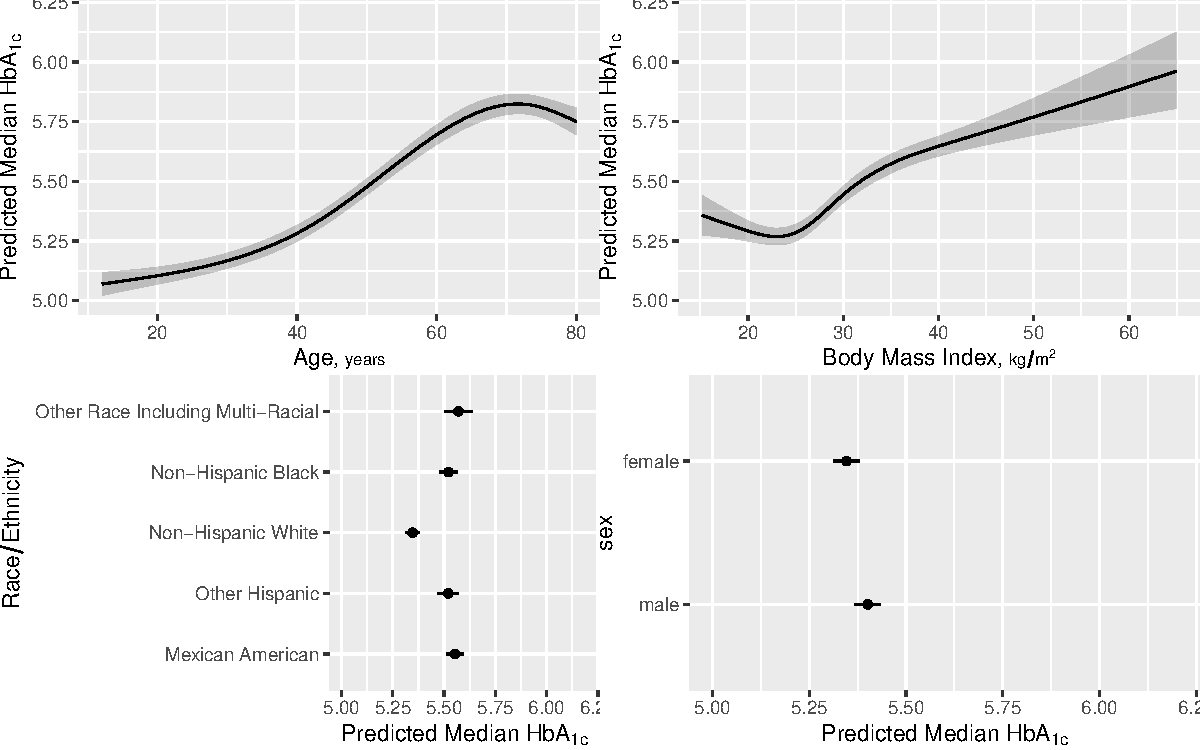
\includegraphics[width=\maxwidth]{descript-rmsa-1} }

\caption[Partial effects in NHANES HbA1c model]{Partial effects in NHANES HbA1c model}\label{fig:descript-rmsa}
\end{figure}

An effect chart is in Fig.~\ref{fig:descript-rmsb} and a nomogram is
in Fig.~\ref{fig:descript-rmsc}.  See
\url{http://stats.stackexchange.com/questions/155430/clarifications-regarding-reading-a-nomogram}
for excellent examples showing how to read such nomograms.
\begin{Schunk}
\begin{Sinput}
plot(summary(f))   # Fig. (*\ref{fig:descript-rmsb}*)
\end{Sinput}
\begin{figure}[htbp]

\centerline{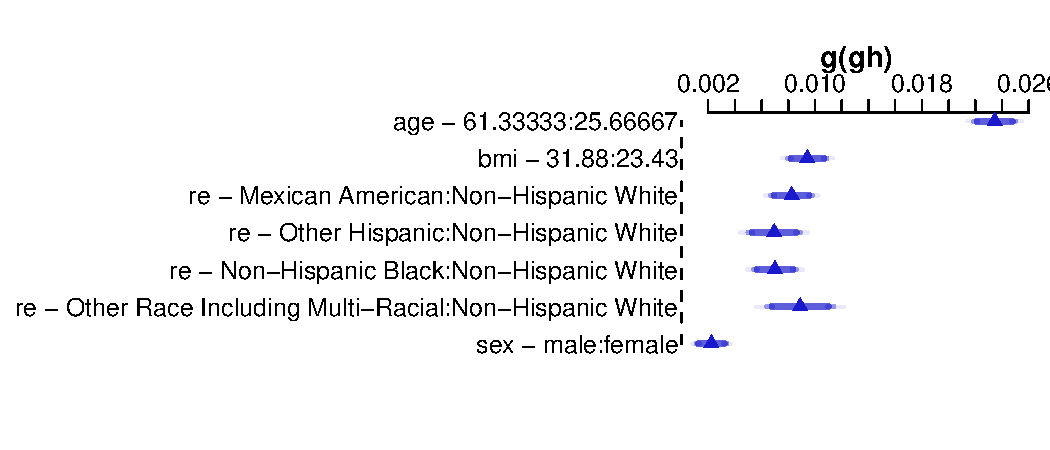
\includegraphics[width=\maxwidth]{descript-rmsb-1} }

\caption[Partial effects chart for transformed glycohemoglobin]{Partial effects chart on the transformed scale.  For age and BMI, effects are inter-quartile-range effects.  0.9, 0.95, and 0.99 confidence limits are shown.}\label{fig:descript-rmsb}
\end{figure}
\end{Schunk}
\begin{Schunk}
\begin{Sinput}
plot(nomogram(f, fun=ginverse, funlabel='Median HbA1c'))  # Fig. (*\ref{fig:descript-rmsc}*)
\end{Sinput}
\begin{figure}[htbp]

\centerline{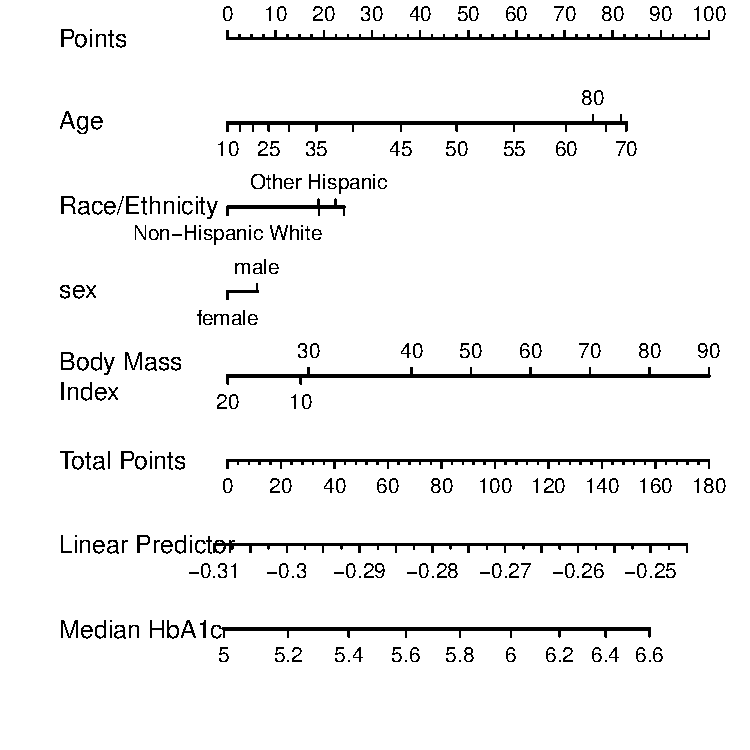
\includegraphics[width=\maxwidth]{descript-rmsc-1} }

\caption[Nomogram for predicting median HbA$_{1c}$]{Nomogram for predicting median HbA$_{1c}$.  To use the nomogram, use the top \Co{Points} scale to convert each predictor value to a common scale.  Add the points and read this number on the \Co{Total Points} scale, then read down to the median.}\label{fig:descript-rmsc}
\end{figure}
\end{Schunk}

\subsubsection{Graphing Effect of Two Continuous Variables on $Y$}
The following examples show the estimated combined effects of two
continuous predictors on outcome.  The two models included interaction
terms, the second example using penalized maximum likelihood
estimation with a tensor spline in diastolic $\times$ systolic blood pressure.

\begin{figure}[!htbp]\leavevmode%
 \centerline{\includegraphics[width=.9\textwidth]{image-sepsis}}
 \caption{Estimated median survival time for critically ill adults}
 \alabel{fig:descript-image-sepsis}
 \end{figure}

\begin{figure}[!htbp]\leavevmode%
 \centerline{\includegraphics[width=.9\textwidth]{image-stroke}}
 \caption[Probability of hemorrhagic stroke vs.\ blood
 pressures]{Logistic regression estimate of probability of a
   hemorrhagic stroke for patients in the GUSTO-I trial given $t$-PA,
   using a tensor spline of two restricted cubic splines and
   penalization (shrinkage).  Dark (cold color) regions are low risk,
   and bright (hot) regions are higher risk.}
 \alabel{fig:descript-image-stroke}
 \end{figure}
 
 Figure~\ref{fig:descript-image-stroke} is particularly interesting
 because the literature had suggested (based on approximately 24
 strokes) that pulse pressure was the main
 cause of hemorrhagic stroke whereas this flexible modeling approach
 (based on approximately 230 strokes)
 suggests that mean arterial blood pressure (roughly a $45^\circ$ line)
 is what is most important 
 over a broad range of blood pressures.  At the far right one can see
 that pulse pressure (axis perpendicular to $45^\circ$ line) may have
 an impact although a non-monotonic one.

\clearpage

\section{Tables} \bmovie{3a}\ddisc{3}
What are tables for?
\bi
\item Lookup of details
\item Not for seeing trends
\item For displaying a summary of a variable stratified by a truly
  categorical variable
\item Not for summarizing how a variable changes across levels of a
  continuous independent variable
\ei

Since tables are for lookup, they can be complex.  With modern media,
a better way to think of a table is as a pop-up when viewing elements
of a graph.

What to display in a table for different types of response variables:
\bi
\item Binary variables: Show proportions first; they should be
  featured because they are normalized for sample size
  \bi
  \item Don't need to show both proportions (e.g., only show
    proportion of females)
  \item Proportions are better than percents because of reduced
    confusion when speaking of percent difference (is it relative or
    absolute?) and because percentages such as 0.3\% are often
    mistaken for 30\% or 3\%.
  \ei
\item Make logical choices for independent and dependent variables. \\
 E.g., less useful to show proportion of males for patients who lived
 vs.\ those who died than to show proportion of deaths stratified by
 sex.
\item Continuous response variables
 \bi
 \item to summarize distributions of raw data: 3 quartiles \\
   recommended format: {\small 35} \textbf{50} {\small 67} or
   35/\textbf{50}/67
 \item summary statistics: mean or median and confidence limits
   (without assuming normality of data if possible)
 \ei
\item Continuous independent (baseline) variables
  \bi
  \item Don't use tables because these requires arbitrary binning
    (categorization) 
  \item Use graphs to show smooth relationships
  \ei
\item Show number of missing values
\item Add denominators when feasible
\item Confidence intervals: in a comparative study, show confidence
  intervals for differences, not confidence intervals for
  individual group summaries
\ei

\begin{table}[!h]
 \caption{Descriptive Statistics: Demographic and Clinical variables\label{summ1}}
 \begin{center}
 \begin{tabular}{lrc}\hline\hline
\multicolumn{1}{l}{}&
\multicolumn{1}{c}{N}&
\multicolumn{1}{c}{ }
\\ \hline
Age&27&{\scriptsize 28~}{\textbf{32} }{\scriptsize 52} \\
C-reactive~protein&27&{\scriptsize  1.0~}{ \textbf{1.8} }{\scriptsize 10.1} \\
Fecal~Calprotectin &26&{\scriptsize  128~}{ \textbf{754} }{\scriptsize 2500} \\
Gender&27&\\
~~~~Female&&0.52~{\scriptsize~$\frac{14}{27}$}\\
Location~of~colitis&27&\\
~~~~Left~side&&0.41~{\scriptsize~$\frac{11}{27}$}\\
~~~~Middle&&0.52~{\scriptsize~$\frac{14}{27}$}\\
~~~~Right~side&&0.07~{\scriptsize~$\frac{~2}{27}$}\\
\hline
\end{tabular}

\end{center}

\noindent {\scriptsize $a$\ }{$\mathbf{b}$\ }{\scriptsize $c$\ } represent the lower quartile $a$, the median $\mathbf{b}$, and the upper quartile $c$\ for continuous variables.\\
$N$\ is the number of non--missing values.\\

\end{table}

See also \href{https://hbiostat.org/talks/rmedicine19.html#18}{hbiostat.org/talks/rmedicine19.html\#18}.
